\documentclass{anstrans}
%%%%%%%%%%%%%%%%%%%%%%%%%%%%%%%%%%%
\title{%
The Nuclear Forensics Problem and Statistical Methods: \\
Evaluating Machine Learning for Spent Fuel Prediction
}
\author{Arrielle C. Opotowsky, Paul P.H. Wilson}

\institute{
Computational Nuclear Engineering Research Group \\
University of Wisconsin at Madison
}

\email{opotowsky@wisc.edu \and paulwilson@wisc.edu}

% Optional disclaimer: remove this command to hide
% \disclaimer{Notice: }

%%%% packages and definitions (optional)
\usepackage{graphicx} % allows inclusion of graphics
\usepackage{booktabs} % nice rules (thick lines) for tables
\usepackage{microtype} % improves typography for PDF
\usepackage{todonotes}

\newcommand{\SN}{S$_N$}
\renewcommand{\vec}[1]{\bm{#1}} %vector is bold italic
\newcommand{\vd}{\bm{\cdot}} % slightly bold vector dot
\newcommand{\grad}{\vec{\nabla}} % gradient
\newcommand{\ud}{\mathop{}\!\mathrm{d}} % upright derivative symbol

\begin{document}
%%%%%%%%%%%%%%%%%%%%%%%%%%%%%%%%%%%%%%%%%%%%%%%%%%%%%%%%%%%%%%%%%%%%%%%%%%%%%%%%
\section{Introduction}

In the event of a nuclear incident, such as the retrieval of stolen nuclear
material or the detonation of a dirty bomb, it is necessary to learn as much as
possible about the source of the materials in a timely manner. In the case of
non-detonated special nuclear material, knowing the reactor parameters that
produced it can point investigators in the right direction in order to
determine the chain of custody of the interdicted material. Determining these
parameters (e.g., cooling time, burnup) requires first characterizing and
calculating certain isotopic ratios, chemical compounds, or trace elements.
Both radiological methods (e.g., gamma spectroscopy) and ionization methods
(e.g., mass spectroscopy) measure these quantities. Although both measurement
techniques have a multitude of techniques within them and thus varying
strengths and weaknesses, the main tradeoff is between time/cost and amount of
information gained. 

The results of these analytic techniques are then compared against existing
databases to obtain the desired reactor parameters. These databases are highly
multidimensional, and furthermore, are rife with missing data entries and
inconsistent uncertainties. Direct comparison between measurement results and a
database therefore may not yield accurate results. Thus, computational
techniques have been developed by nuclear engineers to calculate the parameters
relevant to nuclear forensics analysis. \todo{Cite inverse stuff, possibly
adjoint?} Another approach requiring minimal domain knowledge is the use of
statistical methods via machine learning algorithms. These algorithms can
create a model using the database entries that enables "filling between the
lines" of its entries. Additionally, having a machine-learned model may
overcome the above challenges of multidimensionality, missing data, and
irregular uncertainty.

While different machine learning algorithms and parameters will be
investigated, it is first important to determine if statistical methods can
overcome the inherent database deficiencies. Thus, this paper focuses on
probing the amount of information required to obtain realistic results.  This
can be best understood as the analgous real-world scenario. Although mass
spectroscopy techniques provide extremely accurate isotopic information, they
are time-consuming and more expensice. And although gamma spectroscopy can give
extremely fast results cheaply, it only measures certain radiological signals
and is influenced by many environmental factors, storage, and self-attenuation.

\todo{assumes previous section on fuel cycle sim} In the simulation and machine
learning paradigm, we need to determine what exactly is needed to train a
machine-learned model. Of interest to an entity trying to create a weapon is
partially irradiated fuel if they have plutonium separations capabilities or
any radioactive substance in the case of a dirty bomb. Addressing the former,
we used a set of simulations of spent nuclear fuel at different burnups and
cooling times. 

Can the algorithm overcome the deficiencies of gamma detection and still
provide useful results? Or does it need more information, e.g., exact
isotopics? Thus, ultimately, the goal is to answer the question \textit{How
does the ability to determine forensic-relevant spent nuclear fuel attributes
degrade as less information is available?}. 

But first, we must establish some baseline expectations of reactor parameter
prediction and algorithms to use.  This work is based off previous work on the
subject (cite Dayman) regarding machine learning performace with respect to
information reduction, and expands upon it by also evaluating a more advanced
machine learning algorithm: support vector regression. Below is a more in depth
discussion of nuclear forensics and how machine learning can contribute to this
research area. After that, an experimental design is outlined. Lastly, the
results are presented and discussed. 

%%%%%%%%%%%%%%%%%%%%%%%%%%%%%%%%%%%%%%%%%%%%%%%%%%%%%%%%%%%%%%%%%%%%%%%%%%%%%%%%
\section{Background and Theory}

\subsection{Nuclear Forensics}

The process of nuclear forensics includes the analysis and interpretation of
nuclear material to determine its history, whether that be intercepted spent
nuclear fuel, uranium ore concentrate, or the debris from an exploded nuclear
device. After the technical portion is complete, intelligence data can be used
to aid in material attribution; this is the overall goal of nuclear forensics. 

This study focuses on non-detonated materials, specifically, spent nuclear
fuel. It is important to determine if some intercepted material is from a
commercial fuel cycle or if it is meant for weapons production (and where the
material was obtained from). 

\todo{Workflow for determining SNF quantities of interest}: measure material, use
isotope content and/or isotope ratios to determine things like reactor type,
fuel type and enrichment at beginning of irradiation, cooling time, burnup.
(Classification, Characterization, Interpretation (Analysis), Reconstruction
(Attribution) - from the New Nuclear Forensics book) (Char methods to get
isotopic ratios or use S/ML, Interp examples) After the material
characteristics are measured, they are matched in a forensics database that
includes some or all this information for pre-existing/pre-measured SNF. These
databases are kept by individual countries, and a given database will have
widely varying uncertainty depending where the material was measured as well as
missing data in some fields.  Therefore, matching can be difficult.

A lofty goal for the forensics community would be to develop methods that
provide instantaneous information that is reliable enough to guide an
investigation (e.g., within 24 hours). Fast measurements to provide isotopic
ratios to calculate the above-mentioned fuel parameters of interest would
provide this via some form of a handheld detector that measures gamma spectra.
However, while this nondestructive analysis is rapid, it is also difficult to
evaluate because of the presence of overlapping peaks.  Thus, gamma spectra
give less information at a higher uncertainty than the near-perfect results of
some destructive mass spectroscopy techniques, like TIMS\todo{find MS technique
and citation}.  Additionally, within gamma spectroscopy techniques (e.g., field
vs. lab detectors), uncertainties can vary significantly because of the
detector reponse, environment, storage, electronics, etc.  However, using a
well-trained machine-learned model may be able to overcome these inherent
issues with gamma spectra. The current and future work of this study is
designed with this in mind. 

\subsection{Machine Learning}

Given imperfect data with varying amounts of uncertainty as well as the
required comparison to highly multidimensional databases with missing entries,
many have begun considering computational approaches to nuclear forensics
problems, such as the INDEPTH\todo{cite and discuss}

Another approach utilizes artificial intelligence to solve nuclear forensics
problems, such as implementing searching algorithms for database comparison and
machine learning for determining spent fuel characteristics \todo{cite
hungarian guy, viz guy, dayman paper}.  A variety of statistical and machine
learning tools have been used to characterize spent fuel by predicting
categories or labels (reactor type, fuel type) as well as predicting values
(burnup, initial enrichment, or cooling time) The former uses classification
algorithms and the latter uses regression algorithms. Many algorithms can be
applied to both cases.

A typical (supervised) machine learning workflow would take a set of training
data with labels or values inserted into some statistical learner, calculate
some objective, minimize or maximize that objective, and provide some model
based on that output. Then a test set (with known values) is provided to the
model so that its performance can be evaluated and finalized. After model
finalization, a user can provide a single instance and a value can be predicted
from that. \todo{insert ML schematic}

To obtain reliable models, one must 1. choose/create a training set carefully
and 2. study the impact of various algorithm parameters on the error. Many
algorithms are developed on an assumption that the training set will be
independent and identially distributed (i.i.d.). [Aside: there are ways to
handle skewed data sets] This is important so that the model does not overvalue
or overfit a certain area in the training space. Additionally, algorithm
performance (or error) can be optimized with respect to training set size,
number of features, or algorithm parameters (regularization terms, etc).  These
are known as diagnostic plots. When plotting the training and testing error
with respect to the number of instances, this is known as a learning curve.
When plotting these errors with respect to the number or features or algorithm
parameters, this is known as a validation curve. \todo{insert example
diagnostic plot?}

Algorithm choice is usually based on what is being predicted and intuition
regarding strengths and weaknesses.  For the sake of comparison (i.e. weak
validation), some machine learning approaches here are based on previous
work\todo{cite dayaman} while also extending to a more complex model via an
algorithm that is known to handle highly dimensional data sets well. Thus, this
paper investigates three regression algorithms: nearest neighbor, ridge, and
support vectors.

\subsubsection{Nearest Neighbor Regression}

\todo{intro, alg math, etc} 

Nearest neighbor regression calculates a value based on the instance that is
closest to it. The metrics for distance differ, but in this study, Euclidian
distance was used. There is no learning in this regression, per se; the
training set populates a space and the testing set is compared directly to
that. 

\subsubsection{Ridge Regression}

\todo{intro, alg math, etc} 

Ridge regression utilizes normal linear least squares regression, but with a
parameter that penalizes correct answers to prevent overfitting, which is
referred to as regularization. 

\subsubsection{Support Vector Regression}

\todo{add schematics from pres...or diff pics with the math?} 


Support vector regression (SVR) is an extension of the popular classification
algorithm, support vector machine (SVM).  This algorithm was chosen because of
its ability to handle highly dimensional data well, which in this study is
approximately 300 features. 

SVM classifies two classes by determining an optimal hyperplane, given by wx+b,
between them.  As seen in Figure ?, the algorithm evaluates the quality of the
line that separates two classes by maximizing the width of the margin given the
contraints surrounding the line.  Some problems are not linearly separable, and
thus a penalty term is introduced to allow for misclassifications. As shown in
Figure ?, the algorithm then simultaneously minimizes the misclassifications
while maximizing the margin. 

This can be extended easily to multidimensional analysis via what is called the
\textit{kernel trick}.  First, using a nonlinear kernel function maps the data
into higher dimensional feature space. Then the algorithm can find a linear
separation in this space, as shown in Figure ?. Further, this can be upgraded
from classification to SVR by doing similar math but instead minimizing the
margin, as shown in Figure ?. 

The kernel chosen for this study is the Gaussian radial basis function, shown
below. This has two tuneable parameters, gamma and C. Gamma influences the
width of influence of individual training instances, and strongly affects the
fitting of the model. Low values correspond to underfitting because the
instances have too large of a radius (low influence) and high values correspond
to overfitting because the instances have a small radius (high influence). 

The C parameter also affects the fitting of the model by allowing more or less
support vectors, corresponding to more or less misclassification. A lower C
smooths the surface of the model by allowing more misclassifications, whereas a
higher C classifies more training examples by allowing fewer
misclassifications. Too low and too high of a C can cause under- and
overfitting, respoectively. 

Since there is a tradeoff of fitting strength provided by both parameters, it
is common to run the algorithm on a logarithmic grid from 10'-3 to 10'3 for
each parameter. If plotted on a heatmap of accuracies given gamma and C, there
will be a diagonal of ideal combinations that emerges. The lowest of these is
usually chosen. 


%%%%%%%%%%%%%%%%%%%%%%%%%%%%%%%%%%%%%%%%%%%%%%%%%%%%%%%%%%%%%%%%%%%%%%%%%%%%%%%%
\section{Experimental Design}

\subsection{Testing and Training Sets}

This work begins by simulating the training and test sets described in ref
(cite Dayman). As with the previous work, this will be done using SCALE 6.2
\todo{cite}. Specifically, the ARP module of the activation and depletion code
ORIGEN was used. \todo{add deets and citations}

\todo{show table of training set space}
The parameters of the training set are defined as follows. A smaller burnup
than is typical for spent fuel from a commercial reactor is used in the
previous work likely because stolen fuel pins for weapons use would not likely
be at the end of their lifetime, as the plutonium of interest has decreased by
then. A truly i.i.d. training set would go beyond this, but this is purely for
demonstration with a single use case in mind. 

\todo{show table of test set space}
The previous work also used an external test set, designed to have values in
between the trained values of burnup. This is implemented in this study but it
is expected that cross-validation will better indicate the model performance.
More specifically, using k-fold cross-validation is a common method to use in
the application of machine learning to create more confidence in the resulting
model. \todo{either explain or cite cross validation next}

\subsection{Information Reduction}

The study does evaluate the impact of randomly introduced error of varying
amounts on the ability of the algorithms to correctly predict the burnup. It
also varies the amount of nuclides given as training to the algorithms (a full
list, a short list determined by PCA, and fission products only). However,
machine learning algorithms are heavily dependent on the inputs and parameters
given to them, such as training set sizes, learning rates, etc. Additionally,
it does not consider more advanced aglorithms. This paper adds in the
comparison of the simpler algorithms to neural nets. It also presents learning
curves for each algorithm to investigate the effect of the training set size on
prediction error. For the classification of reactor type, ROC curves are also
presented to evaluate prediction and generalization strength. For the
regression of burnup, ??? pairwise t test?.  Thus, I will first investigate
these algorithms with no error introduced, but will extend the validation from
a predetermined test set to be randomly partitioned cross validation.  And the
next study will introduce error by limiting the nuclides to only those that can
be measured with a gamma spectrometer (future work).

\subsection{Algorithm Evaluation}

Using predetermined test set:

1. Learning curves: For a given (randomly chosen) training set size for each
algorithm, run several trainings and predictions. This helps determine if we
are over or under training and each algorithm's robustness to over/under
fitting.  

2. Regression Training Error: Confidence intervals on predictions to understand
true error versus sample error Test set must be > 30 instances, Can easily
calculate N\% confidence interval.

Using cross-validation instead:

1. redo learning curve study without having to run several trainings and
predictions for each set (bc that's already done!)

2. redo confidence interval study


\subsection{Comparing Algorithms}

Maybe can delete this if I already discuss it in the above section. Options for
comparison of algorithms: Comparing classification of 2 classes on same ROC
plot with multiple ML systems, Scatter plots, Pairwise t-tests. 

%%%%%%%%%%%%%%%%%%%%%%%%%%%%%%%%%%%%%%%%%%%%%%%%%%%%%%%%%%%%%%%%%%%%%%%%%%%%%%%%
\section{Results and Analysis}

1. Learning curve
2. Validation curve
3. Random error curve

Want to show the difference between test/train error plots and CV/train error
plots.  Determine some argument that perfers the latter. For the above
categories in the validation section, can show plots directly next to each
other (for 1, 2, 3) to hopefully show that cross validation provides better
generalizability.

\todo{Discuss understanding confidence intervals in predictions.}

\section{Notes from Meeting Regarding Signatures}
\subsection{U Processing Signatures}
Isotopics provide the following: 
1. Enrichment indicators
2. radiochronometers provide info on separations, metal, etc
3. heterogeneity of isotopics provide info on blending
4. stable isotopes/atmosphere 
Chemical characteristics ask: 
1. chemical products and trace contaminants @ each step
2. aging in different atmospheres
Processing Signatures in particular:
Shifting focus towards U metals


\subsection{Pu Processing Signatures}

%%%%%%%%%%%%%%%%%%%%%%%%%%%%%%%%%%%%%%%%%%%%%%%%%%%%%%%%%%%%%%%%%%%%%%%%%%%%%%%%
%\subsection{Subsection Goes Here}
%The user must manually capitalize initial letters of a subsection heading.
%
%For those who like equations in their papers, \LaTeX\ is a good choice. Here is
%an equation for the Marshak diffusion boundary condition:
%\begin{equation} \label{eq:marshak}
%  4 J^- = \phi + 2 D \vec{n} \vd \grad \phi \,.
%\end{equation}
%If we so choose, we can effortlessly reference the equation later.
%
%Another paragraph starts with Eq.~\eqref{eq:marshak} and sets $J^-$ to zero, a
%vacuum boundary condition:
%\begin{equation*}
%  0 = \phi + \frac{2}{3} \frac{1}{\sigma} \vec{n} \vd \grad \phi \,.
%\end{equation*}
%The extrapolation distance is $2/3$. A more detailed asymptotic analysis yields
%an extrapolation distance of about $0.71045$.
%
%Figure~\ref{fig:voltage} shows how a plot might conceivably look in your
%document. Always place figures after they are referenced so as not to throw
%off the reader. You can use symbols and different line styles to help
%differentiate your results, especially if they are printed in black and white.
%Note how Fig.~\ref{fig:voltage} uses dashed lines \verb|--| for the exact
%solution, solid lines \verb|-| for the new method's solutions, and dotted lines
%\verb|:| for existing inaccurate methods.
%\begin{figure}[ht] % replace 't' with 'b' to force it to be on the bottom
%  \centering
%  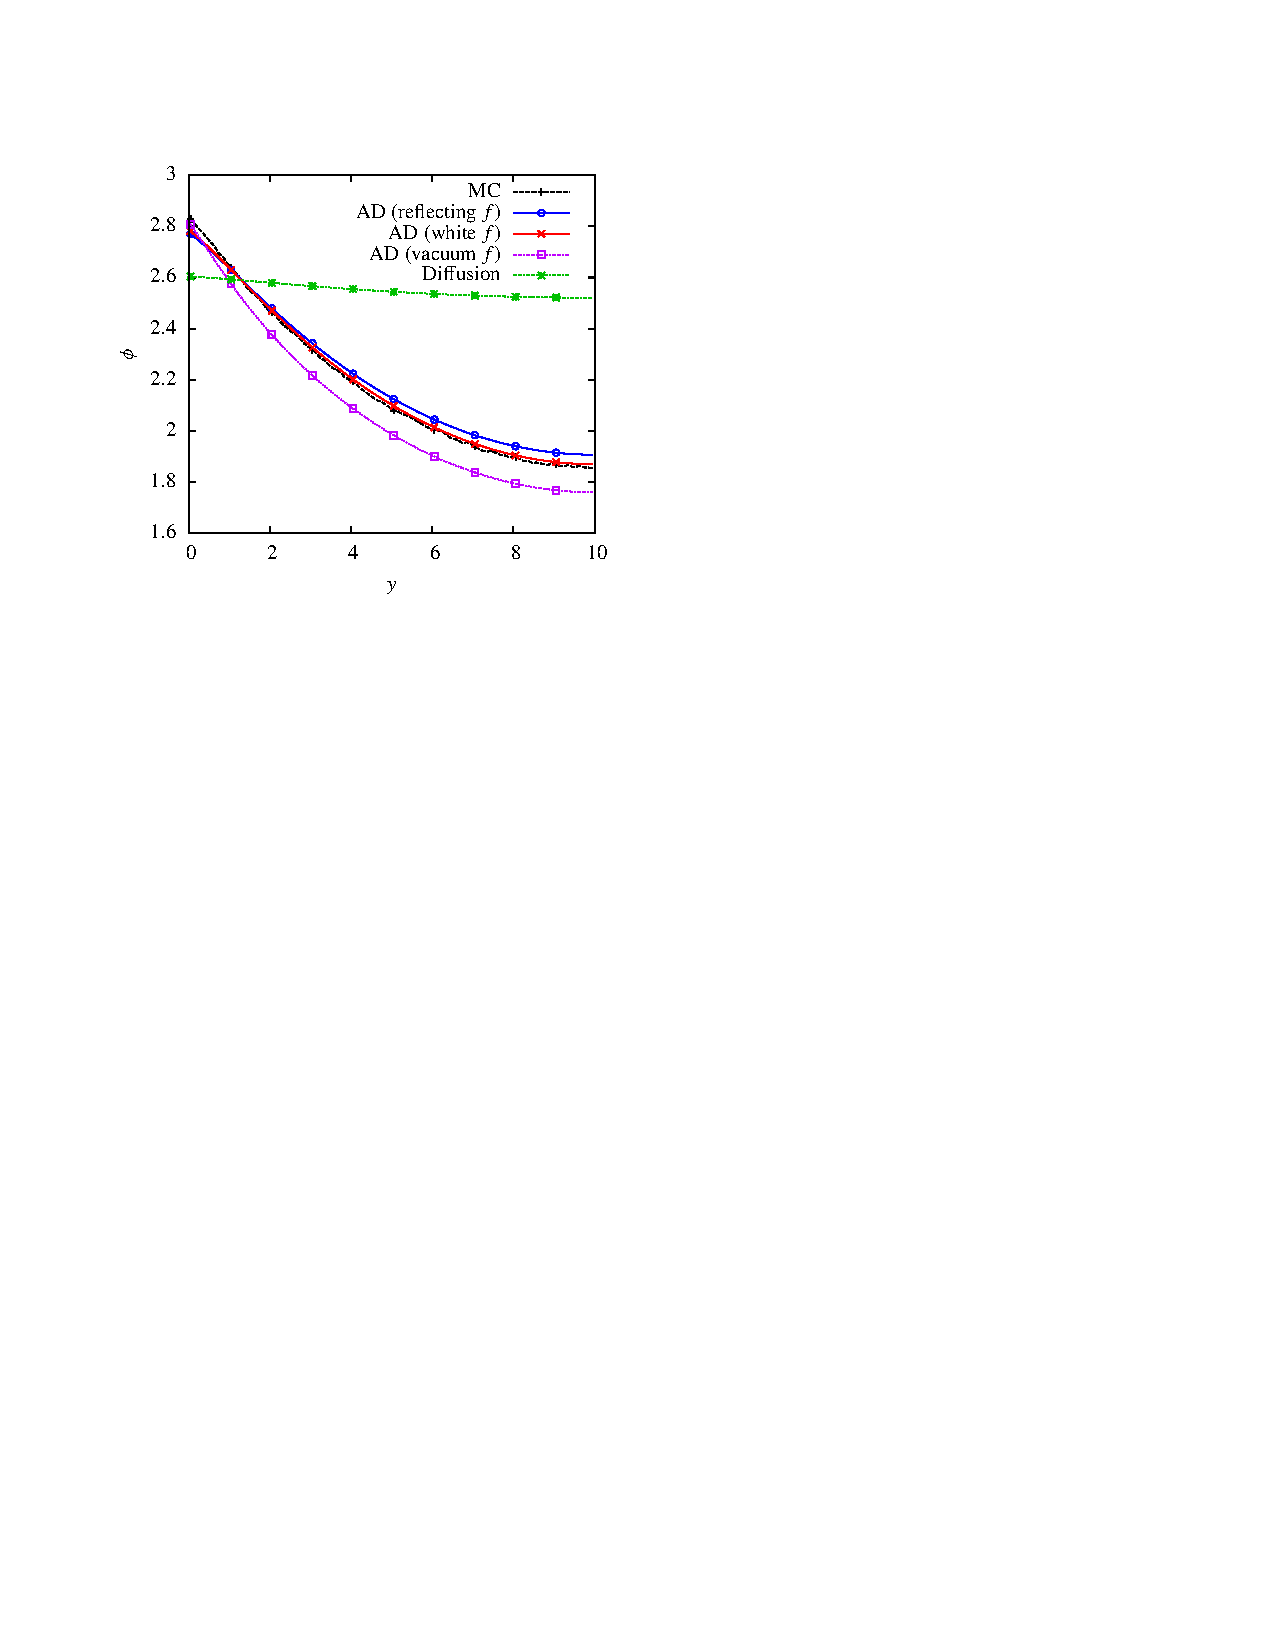
\includegraphics{example_figure}
%  \caption{Captions are flush with the left.}
%  \label{fig:voltage}
%\end{figure}
%
%Later on, we can include a table, even one that spans two columns such as
%Table~\ref{tab:widetable}.
%%%%%%%%%%%%%%%%%%%%%%%%%%%%%%%%%%%%%%%%%
%\begin{table*}[htb]
%  \centering
%\begin{tabular}{llllllllll}\toprule
%      & $\phi_T(0)$      & $\phi_T(10)$      & $\phi_T(20)$      &
%      $\phi_D(0)$      & $\phi_D(10)$      & $\phi_D(20)$      & $\rho$      &
%      $\varepsilon$      & $N_\text{it}$
%\\ \midrule
%$c=0.999$  & 0.9038 & 20.63 & 31.24 & 0.9087 & 20.63 & 31.23 & 0.2192 & $10^{-7}$ & 15
%\\
%$c=0.990$  & 0.3675 & 13.04 & 24.7 & 0.3696 & 13.04 & 24.69 & 0.2184 & $10^{-7}$ & 15
%\\
%$c=0.900$  & 0.009909 & 4.776 & 17.64 & 0.009984 & 4.786 & 17.63 & 0.2118 & $10^{-7}$ & 14
%\\
%$c=0.500$  & $6.069\times 10^{-5}$ & 2.212 & 15.53 & 6.213$\times 10^{-5}$ & 2.239 & 15.53 & 0.2068 & $10^{-7}$ & 13
%\\
%\bottomrule
%\end{tabular}
%  \caption{This is an example of a really wide table which might not normally
%  fit in the document.}
%  \label{tab:widetable}
%\end{table*}
%%%%%%%%%%%%%%%%%%%%%%%%%%%%%%%%%%%%%%%%%
%Notice how the table reference uses a Roman numeral
%for its numbering scheme, whereas the figure reference uses an Arabic numeral.
%For one-column tables, use the \verb|table| environment; two-column tables use
%\verb|table*|. The same applies to figures.
%
%%%%%%%%%%%%%%%%%%%%%%%%%%%%%%%%%%%%%%%%%%%%%%%%%%%%%%%%%%%%%%%%%%%%%%%%%%%%%%%%%
%\subsection{Another Subsection}
%Excessive sectioning in a three-page document is discouraged, but here are more
%subsections to demonstrate compliance with the ANS formatting guidelines.
%
%\subsubsection{Third-level Heading}
%This subsubsection shows compliance with the ANS-specified standard. This level
%of heading should be used rarely.
%
%\subsubsection{Another Such Heading}
%And, if you really think you need a third-level heading, you should make sure
%that your subsection needs at least two of them.
%
%%%%%%%%%%%%%%%%%%%%%%%%%%%%%%%%%%%%%%%%%%%%%%%%%%%%%%%%%%%%%%%%%%%%%%%%%%%%%%%%%
%\section{Conclusions}
%
%The included ANS style file and this clear example file are a panacea for
%the hours of headache that invariably results from formatting a document in
%Microsoft Word.
%
%%%%%%%%%%%%%%%%%%%%%%%%%%%%%%%%%%%%%%%%%%%%%%%%%%%%%%%%%%%%%%%%%%%%%%%%%%%%%%%%%
%\appendix
%\section{Appendix}
%
%Numbering in the appendix is different:
%\begin{equation} \label{eq:appendix}
%  2 + 2 = 5\,.
%\end{equation}
%and another equation:
%\begin{equation} \label{eq:appendix2}
%  a + b = c\,.
%\end{equation}

%%%%%%%%%%%%%%%%%%%%%%%%%%%%%%%%%%%%%%%%%%%%%%%%%%%%%%%%%%%%%%%%%%%%%%%%%%%%%%%%
\section{Acknowledgments}
This material is based upon work supported a Department of Energy Nuclear
Energy University Programs Graduate Fellowship.

%%%%%%%%%%%%%%%%%%%%%%%%%%%%%%%%%%%%%%%%%%%%%%%%%%%%%%%%%%%%%%%%%%%%%%%%%%%%%%%%
\bibliographystyle{ans}
\bibliography{bibliography}
\end{document}

